%This is a \LaTeX\  template created following the Project Report Guidelines of the Examination Office at the International University of Applied Sciences. Please review carefully if all the details in this template are the same as those stated in the official guidelines. Always follow the official guidelines first rather than this template. If you find inconsistencies between the official guideline and this template, please report them to gissel.velarde@iu.org.
%Author: Gissel Velarde

\documentclass[11pt,a4paper]{article}

%\usepackage[margin=2cm]{geometry} % full-width
\usepackage[left=2cm,right=2cm,top=2cm,bottom=2cm]{geometry}
\usepackage[utf8]{inputenc}

\usepackage{setspace}
\onehalfspacing % Set line spacing to 1.5

\usepackage{helvet} %arial font
\renewcommand{\familydefault}{\sfdefault}

\usepackage{sectsty}
\usepackage{graphicx}

\usepackage[hidelinks]{hyperref} 
\usepackage{apacite} %APA style citation, make sure it comes after hyperref!

\usepackage{amsmath, amssymb, latexsym}

%packages for drawings
\usepackage{tikz}
\usetikzlibrary{decorations.pathreplacing}
\usetikzlibrary{fadings}

\usepackage{parskip} %https://www.overleaf.com/learn/latex/Articles/How_to_change_paragraph_spacing_in_LaTeX

%\usepackage[style=apa, backend=biber]{biblatex}
%\addbibresource{references.bib}

\setlength\parindent{0pt} %https://tex.stackexchange.com/questions/27802/set-noindent-for-entire-file

%\usepackage{ragged2e} %justified
%\justifying


\title{PROJECT PROPOSAL TEMPLATE}
\author{ Gissel Velarde }
%\date{\today}

\begin{document}

\maketitle	

% TOC
 \tableofcontents
 \pagebreak
\begin{abstract}
(200 words maximum) The abstract should state the motivation, that is, why the study will be done or which problem will be addressed, which method will be used, as well as the expected results and contributions or implications of the work. Give details. See for example the abstract in \cite{krizhevsky2017imagenet}.
\end{abstract}


%--Paper--
\section{Graphical abstract}

\begin{figure}[h]
	\centering
	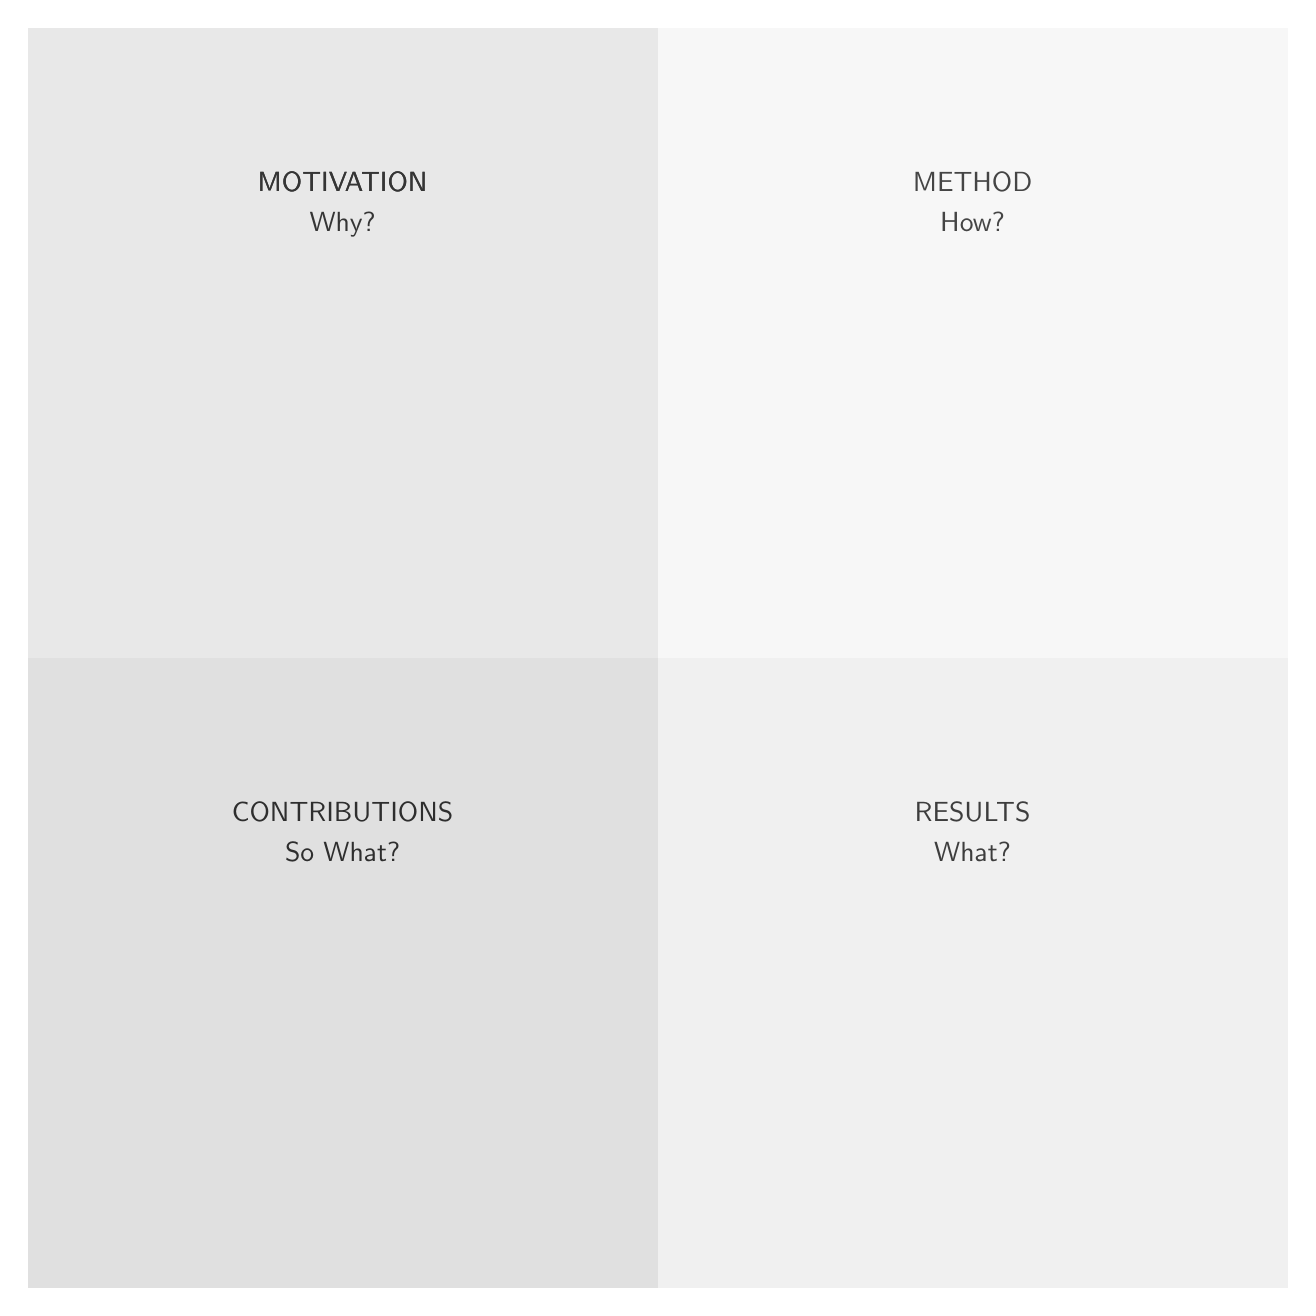
\begin{tikzpicture}
		\node at (4,14){\begin{tabular}{c}MOTIVATION\end{tabular}};	
		
		\node at (4,14){\begin{tabular}{c}MOTIVATION\end{tabular}};	
		\node at (4,13.5){\begin{tabular}{c}Why?\end{tabular}};
		
		\node at (12,14){\begin{tabular}{c}METHOD\end{tabular}};
		\node at (12,13.5){\begin{tabular}{c}How?\end{tabular}};		
				
		\node at (12,6){\begin{tabular}{c}RESULTS\end{tabular}};
		\node at (12,5.5){\begin{tabular}{c}What?\end{tabular}};
			
		\node at (4,6){\begin{tabular}{c}CONTRIBUTIONS\end{tabular}};
		\node at (4,5.5){\begin{tabular}{c}So What?\end{tabular}};
		
		\fill[black!30!white, fill opacity=0.3] (0,16) rectangle (8,8);
		
		\fill[black!10!white,fill opacity=0.3] (16,16) rectangle (8,8);
		
		\fill[black!40!white,fill opacity=0.3] (0,0) rectangle (8,8);
		
		\fill[black!20!white,fill opacity=0.3] (16,0) rectangle (8,8);				
		
		\end{tikzpicture}
	\caption[Graphical Abstract]{Graphical Abstract. Include a graphical abstract of the proposal with the motivation, method, expected results and contributions. Examples of graphical abstracts can be found in \shortcite{graphicalabstract, VELARDE2024a}. }
	\label{fig:1}
\end{figure}

\newpage
\section{The State-of-the-art}
(100 words maximum, 4 research papers minimum) Describe and reference the state-of-the-art, primarily focussing on peer-reviewed scientific publications. Explain how these works relate to your proposal. Use the American Psychological Association (APA) style for citations \shortcite{hughes2017APA}.

\section{Objectives}
(150 words maximum) Describe the main objective and sub-objectives of the project. Alternatively propose a hypothesis and its research questions. 

\section{The method}
(150 words maximum, 1 Figure) Describe the intended method, techniques, and evaluation framework. Include a Figure that explains the intended method. See for example Figure 1 in \shortcite{Sossi-Velarde-Zieba}, or Figure 2 in \shortcite{Badrinarayanan}.

\subsection{Data}
(Minimum 1 Dataset) List and describe the dataset or datasets to be used.

\section{The plan}
Include a Gantt chart with tasks and their expected duration. 

\section{Expected Contributions}
(Maximum 5 sentences of less than 25 words each) List 5 expected contributions of your proposed project.
 
\section{Agreements and constraints}
(100 words maximum) State if: 

\begin{itemize}
\item the work can be published without restrictions, or 
\item if it needs a confidentiality agreement.
\item In addition, mention the stakeholders if any.
\end{itemize}

%the bibliography
\bibliographystyle{apacite}
\bibliography{references.bib}

%--/Paper--

\end{document}